\documentclass{article}
\usepackage[utf8]{inputenc}
\usepackage{graphicx}
\usepackage{amsmath}
\usepackage{hyperref}
\usepackage[a4paper, textwidth=450pt]{geometry}

\graphicspath{ {./files/} }

\title{O17e Diffraction Report}
\author{Adam Kit}
\date{May 2020}


\begin{document}

\maketitle

\section{Preperation}
In order to understand diffraction, we make use of the Fourier transform. This allows us to predict how and where light will arrive when traveling through an aperature. Instead of using Origin, I chose to work using python, utelizing the pandas, numpy, and scipy libraries. I justify my choice by the fact that I will have to greatly depend on these libraries if I am to work in the simulation field of study, so I must begin now my preperation. All graphs are then made with matplotlib, and the github repository for each Lab can be found  \href{https://github.com/fusionby2030/Numerical_Methods/tree/master/Labs/017E}{here.} I note that this report mainly focuses on the expiremental questions given in the Powerpoint presentation for the Virtual Lab Course.\\
\subsection{Fourier Transforms}

\begin{figure}[h]
  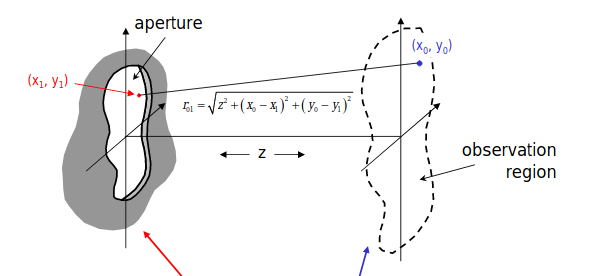
\includegraphics[scale=0.5]{fraunhofferdiffraction.png}
  \caption{Here the light in the far field (blue line and variables) is simple the fourier transform of the apertured field (red line and variables)}
\end{figure}


The Fourier transform of a function $f(x)$ is defined as:
$$ F(k) = FT[f(x)]=\int_{-\infty}^{\infty}f(x)e^{-2\pi ikx} dx$$
\\
The single slit function is defined as:

\[
f(x) =
  \begin{cases}
    \text{1,} &\quad\text{if -b/2}\le\text{x}\le\text{b/2} \\
    \text{0,} &\quad\text{otherwise}
  \end{cases}
\]

and our Fourier transform becomes:

$$F(k) = \int_{-\infty}^{\infty}f(x)e^{-2\pi ikx}dx = \int_{-b/2}^{b/2}e^{- 2\pi ikx}dx = \frac{e^{\pi ikb}-e^{-\pi ikb}}{2\pi ik} = \frac{sin(\pi kb)}{\pi k} = bsinc(\pi bk) $$


For the double slit, the following domain is used:

\[
f(x) =
  \begin{cases}
    \text{1,} &\quad\text{if -(g+b)/2}\le\text{x}\le\text{-(g-b)/2} \\
     &\quad\text{or (g-b)/2}\le\text{x}\le\text{(g+b)/2} \\ \\
    \text{0,} &\quad\text{otherwise}
  \end{cases}
\]

And using the law of displacements
$$ \int_{-\infty}^{\infty} f(x-g)e^{-2\pi ikx}dx = \int_{-\infty}^{\infty} f(x)e^{-2\pi ik(x+g)} dx = e^{-2\pi ig k} F(k) $$

The new transform turns out to be
$$ F(k) = \big( e^{2\pi i gk} + e^{-2\pi i gk}\big)b\operatorname{sinc}(b\pi k) = 2b\cos(2\pi gk)\operatorname{sinc}(b\pi k) $$

\subsection{Fraunhoffer Diffraction Patterns}
For the single slit, we have the equation for the electric field at a point on a screen defined as:

$$E(\beta) = \frac{bE_0}{2\pi}\frac{sin(\beta)}{\beta}  $$

where $\beta = bk/2$. Not surprisingly, this is very similar to the Fourier Transform we found above.


\subsection{Fast Fourier Transform}
I use a self made python function used to calculate the fast fourier transform of a given function, where I implement the Cooley and Turkey method:

\begin{align}
X_k &= \sum_{n=0}^{N-1} x_n \cdot e^{-i 2\pi k n / N} \\
    &= \sum_{m=0}^{N/2-1}x_{2m} \cdot e^{-i 2\pi k (2m) / N} +\sum_{m=0}^{N/2-1}x_{2m+1} \cdot e^{-i 2\pi k (2m+1) / N} \\
    &= \sum_{m=0}^{N/2-1}x_{2m} \cdot e^{-i 2\pi k m / (N/2)} + e^{-i 2\pi k / N} \sum_{m=0}^{N/2-1}x_{2m+1} \cdot e^{-i 2\pi k m / (N/2)}
\end{align}

Where $X_k$ are the values of the fourier transform of a given function defined by the values $x_n$. The python implementation can be found on my github under the file \href{https://github.com/fusionby2030/Numerical_Methods/tree/master/Labs/017E/fastfouriertransform.py}{\textit{fastfouriertransform.py}}.

Interestingly enough, the FFT is a direct implementation of the convolution theorem for the fourier transform. The convolution theorem:
$$FT[f(x) \otimes g(x)] = FT[\int_{-\infty}^{\infty} f(x')g(x-x')dx'] = FT[f(x)]FT[g(x)]=F(k)G(k) $$

where for the FFT, the functions x and y are functions of discrete variable sequences.
$$x\otimes y = FFT^{-1} [FFT(x) * FFT(y)] $$

which uses the convolution theorem for inverse Fourier transforms!

$$ F^{-1} (f\otimes g) = F^{-1}(f)* F^{-1}(g) $$


\section{Experimental Question 1}
Why does the intensity profile not depend on the distance d between the slits and the camera, if the slide holder position is varied in the range between polarizer and lens?

\subsection{Relationship between intensity and distance}
This is an interesting question since to use the Fraunhoffer diffraction limit we need $d \geq \geq \frac{\pi b^2}{\lambda} $. Thus if we have a slit of width $b = 0.1$cm, visible light must travel more than a kilometer to reach the Fraunhofer limit!

So if we use a lens with focal length $f$ and place it an arbitrary distance L from the slit, the lens would produce an image of the Fraunhofer patter at a new location $p$, following the lens image formula: $$\frac{1}{f} = \frac{1}{-(d-L)}+\frac{1}{p} $$ where d is the distance from slit to camera.

i.ef the Fraunhoffer difraction patter, when in the image system, is a virtual object. Thus at great distances $d \rightarrow \infty$ the Fraunhoffer patter appears at the focus of the lens $p = f$ and thus the spacing between the slit and camera is not playing a big role.
\\
\\
\\
\section{Experimental Question 2}
Compare the single slit intensity profiles in files labelled ES1-1 and ES1-2 The data were taken for two slightly different heights of the camera. What might cause the differences in the observed patterns?

For ES1-1 we see that a maximum value $\approx$ 0.8 is occuring at around the halfway point (1500 pixels), while for ES1-2 we see the max value $\approx0$ 0.7 at slightly before the halfway point (1400 pixels). The height in the camera is causing this, as we know for diffraction, the highest intensity of the diffracted light is occuring on directly on the optical axis. This leads me to believe that the camera recording ES1-1 data was more aligned with the optical axis than the camera record ES1-2 data. However, if we look at the minimums in the graphs, we see that ES1-1 did not register much of anything for the right minimum light intensity. Therefore, I move forward using the ES1-2 data, for it is more suitable for Fourier analysis, and can be seen:



\subsection{Attempt to Reproduce}
We can also produce this kind of graph numerically, which can be found in the github repository under the file \href{https://github.com/fusionby2030/Numerical_Methods/tree/master/Labs/017E/simulatedsingleslit.py}{\textit{simulatedsingleslit.py}}
For the single slit we can define a square slit at the origin of a graph with amplitude $ I_0 = 1 V/ \sqrt{\mu m} $ and width $d=2.5*10^{-6}$ in Figure \ref{Seen}.

\begin{figure}[h]
  \caption{$f(x) = 1$ for $\frac{-b}{2} \le x \leq\frac{b}{2}$}
  \centering
  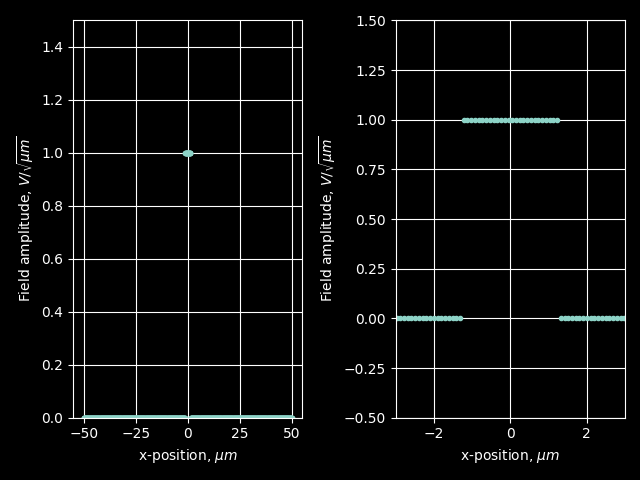
\includegraphics[scale=0.6]{slitrepro.png}
  \label{Seen}
\end{figure}

Then we preform the FFT of the above graphs and compare them to the theory, which is seen in Figure \ref{attempt}. So our simulated values and FFT agree okay. But there is much room for error in the calculation of both, which can lead to discrepencies. For example: aliasing, or rounding errors.
\begin{figure}[h]
  \caption{Theory: $I^2 = \frac{b^2 E_0^2}{\lambda f} sinc^2(\frac{ bx}{\lambda f})$ vs FFT }
  \centering
  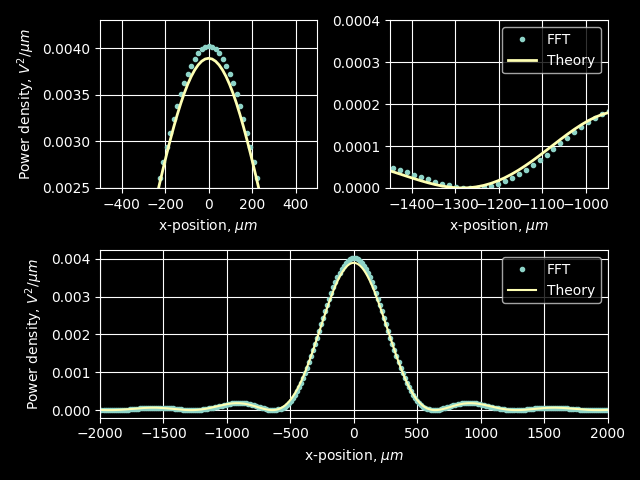
\includegraphics[scale=0.6]{thoeryvsnum.png}
  \label{attempt}
\end{figure}

\section{Experimental Question 3}
Explain the relation between the FFT of the intensity profile and the form and dimensions of the single or double slit. In case of the double slit, how do you read off slit distance and slit width from the FFT pattern?

These graphs were created using numpy and matplotlib and can be found in the file \href{https://github.com/fusionby2030/Numerical_Methods/tree/master/Labs/017E/graphingfunctions.py}{\textit{graphingfunctions.py}}

\subsection{Single Slit}
\begin{figure}[h]
  \caption{Here the FFT of the Single Slit intensity profile is preformed}
  \centering
  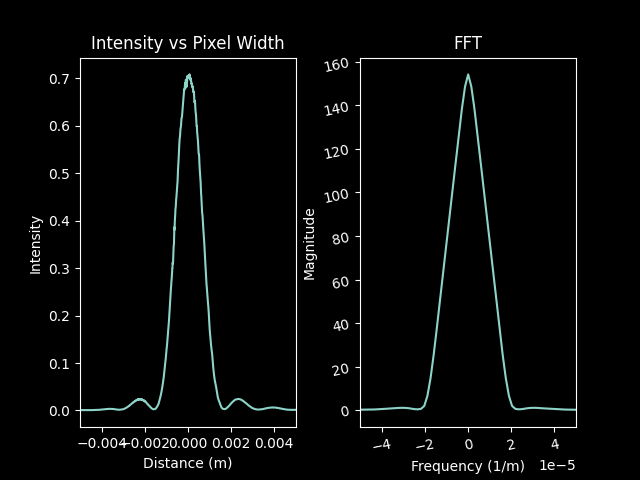
\includegraphics[scale=0.6]{ES1_2graph.png}
  \label{singleslit}

\end{figure}
The FFT in Figure \ref{singleslit} shows the dimensons of the slit by using the equations from the preperation. The width of the FFT of the intensity profile is going to be $2*b$, so we find that $b\approx 2.5*10^{-5}$
\subsection{Double Slit}
\begin{figure}[h]
  \caption{Here the FFT of the Double Slit intensity profile is preformed}
  \centering
  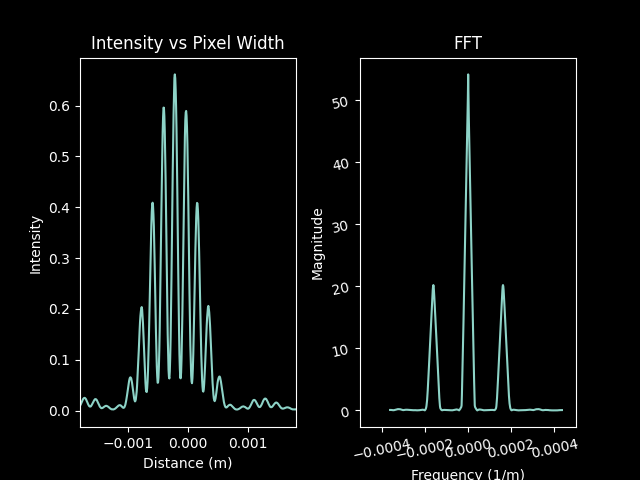
\includegraphics[scale=0.6]{DS4_1graph.png}
  \label{doubleslit}

\end{figure}
In Figure \ref{doubleslit} we see the graph of the Intensity and the FFT for the double slit.
From the preperation, we know that the middle triangle is defined has a width of $2*b$ thus to slit width $b=3.872*10^{-5}$ while the two smaller ones have a width of $2*g$ thus to a slit distance $g=8.55*10^{-4}$, both in units of meters.

\section{Expiremental Question 4}
How is this experiment related to Heisenberg’s uncertainty principle? In case of the single slit, can you make a numerical estimate of the product $\Delta x \Delta p$?

\subsection{Heisenberg’s uncertainty principle}
If we instead considered the width of the slit to not be a static value $d$, but rather as the uncertainty $\Delta x$, we can likewise translate the vector of movement for the light exiting the slit as $ \Delta p$. The electron is gaining momentum in the y direction as it exits, and since $\theta $ is remaining the same,  the single slit diffraction formula becomes: $$sin(\theta) \approx \theta \approx \frac{\lambda}{\Delta x} \approx \frac{\Delta p_y }{p_x}$$

With a wider slit, we would get a smaller diffraction patter, and for a smaller slit, a wider diffraction pattern. This makes sense as if we increase uncertanity in $\Delta x$ (widen the slit) we have a lower uncertanity $\Delta p$ (thinner diffraction pattern), and for the converse, if we decrease uncertainty in $\Delta x$ (decrease slit size) leads to higher $\Delta p$ (wider diffraction pattern).

Using the debroglie relationship for momentum and wavelength: $p_x = \frac{h}{\lambda}$ we see that $$\frac{\lambda}{\Delta x} \approx \frac{\Delta p_y  \lambda}{h} \rightarrow \Delta x \Delta p_y \approx h$$ Although certainly not the equal to the general definition of the principle, $\Delta p_x \Delta x \geq \frac{h}{4\pi} $, we still recieve a decent approximation. Little did Fraunhoffer know...

\section{Additional Material}
What happens when the distance between camera and slit is small such that the Fraunhoferlimit does not apply any more?
\subsection{ Distance }
Well with $\lambda / d \leq \leq 1$ we know that the intereference effects may not be observable.

I made graphs for each file in the additional material which can be found in the githup repository in the folder \href{https://github.com/fusionby2030/Numerical_Methods/tree/master/Labs/017E/FresnelGraphs}{\textit{FresnelGraphs}}.

\begin{thebibliography}{9}
\bibitem{latexcompanion}
James W. Cooley and John W. Tukey
\textit{An algorithm for the machine calculation of complex Fourier series}.
Math. Comp. 19 (1965)

\bibitem{optics}
Brooker, Geoffrey
\textit{Modern Classical Optics}
Oxford: Oxford University Press (2003)
\end{thebibliography}






\end{document}
